\chapter{Supplementary Material}

\section{PGExplainer algorithms}

\begin{algorithm}
    \caption{Training Algorithm for Explaining Node Classification.}
    \begin{algorithmic}[1]
    \REQUIRE Input graph $G_o = (\mathcal{V}, \mathcal{E})$, node features $X$, node labels $Y$, set of instances to be explained $\mathcal{I}$, trained GNN model: $\text{GNNE}_{\Phi_0}(\cdot)$ and $\text{GNNC}_{\Phi_1}(\cdot)$, parameterized explainer MLP $\Psi$.
    \FOR{each node $i \in \mathcal{I}$}
        \STATE $G^{(i)}_o \leftarrow$ extract the computation graph for node $i$.
        \STATE $Z^{(i)} \leftarrow \text{GNNE}_{\Phi_0}(G^{(i)}_o, X)$.
        \STATE $Y^{(i)} \leftarrow \text{GNNC}_{\Phi_1}(Z^{(i)})$.
    \ENDFOR
    \FOR{each epoch}
        \FOR{each node $i \in \mathcal{I}$}
            \STATE $\Omega \leftarrow$ latent variables calculated with (10).
            \FOR{$k \leftarrow 1$ to $K$}
                \STATE $G^{(i,k)}_s \leftarrow$ sampled from (4).
                \STATE $\hat{Y}^{(i,k)}_s \leftarrow \text{GNNC}_{\Phi_1}(\text{GNNE}_{\Phi_0}(G^{(i,k)}_s, X))$.
            \ENDFOR
        \ENDFOR
        \STATE Compute loss with (9).
        \STATE Update parameters $\Psi$ with backpropagation.
    \ENDFOR
    \end{algorithmic}
    \end{algorithm}
    
    \vspace{0.5cm}
    
    \begin{algorithm}
    \caption{Training Algorithm for Explaining Graph Classification.}
    \begin{algorithmic}[1]
    \REQUIRE A set of input graphs with $i$-th graph represented by $G^{(i)}_o$, node features $X^{(i)}$, label $Y^{(i)}$, trained GNN model: $\text{GNNE}_{\Phi_0}(\cdot)$ and $\text{GNNC}_{\Phi_1}(\cdot)$, parameterized explainer MLP $\Psi$.
    \FOR{each graph $G^{(i)}_o$}
        \STATE $Z^{(i)} \leftarrow \text{GNNE}_{\Phi_0}(G^{(i)}_o, X^{(i)})$.
        \STATE $Y^{(i)} \leftarrow \text{GNNC}_{\Phi_1}(Z^{(i)})$.
    \ENDFOR
    \FOR{each epoch}
        \FOR{each graph $G^{(i)}_o$}
            \STATE $\Omega \leftarrow$ latent variables calculated with (11).
            \FOR{$k \leftarrow 1$ to $K$}
                \STATE $G^{(i,k)}_s \leftarrow$ sampled from (4).
                \STATE $\hat{Y}^{(i,k)}_s \leftarrow \text{GNNC}_{\Phi_1}(\text{GNNE}_{\Phi_0}(G^{(i,k)}_s, X^{(i)}))$.
            \ENDFOR
        \ENDFOR
        \STATE Compute loss with (9).
        \STATE Update parameters $\Psi$ with backpropagation.
    \ENDFOR
    \end{algorithmic}
\end{algorithm}

\section{Replication sweeps}
TODO: COMPLETE THESE TABLES!! ONLY CONSIDER NUM-TRAINING OF 30 FOR COMPARABILITY, AS WELL AS NODE SETS USED IN ORIGINAL (Tree-Grid only one where AUC not computabel)!?

\newcolumntype{Y}{>{\centering\arraybackslash}X}
\begin{table}[h]
    \centering
    \scriptsize
    \begin{tabularx}{\linewidth}{|c|c|c|Y|Y|c|c|c|c|Y|}
    \hline
    \multicolumn{10}{|c|}{\textbf{BA-Shapes}} \\ \hline
    entropy reg & epochs & lr\_mlp & sampled graphs & sample bias & seed & size reg & tT & t0 & num training instances \\ \hline
    1.0 & 10 & 0.003 & 1 & 0.0 & - & 0.05 & 0.05 & 1.0 & \text{All} \\ \hline
    1.0 & 10 & 0.003 & 1 & 0.0 & - & 0.05 & 2.0 & 5.0 & \text{All} \\ \midrule
    \textbf{0.1} & 10 & 0.0003 & \textbf{1} & 0.0 & 74 & 0.005 & \textbf{1} & 5.0 & 30 \\ 
    0.5 &  & \textbf{0.003} & 5 &  & 75 & \textbf{0.05} & 2 &  &  \\ 
    1.0 &  &  0.03 & 10 &  & 76 & 0.1 & 5 &  &  \\ \hline
    \end{tabularx}
    \caption[BA-Shapes Sweep]{First row contains the values used in the original code; second row for replication. Highlighted values are the best performing.}
\end{table}


\begin{table}[h]
    \centering
    \scriptsize
    \begin{tabularx}{\linewidth}{|c|c|c|Y|Y|c|c|c|c|Y|}
    \hline
    \multicolumn{10}{|c|}{\textbf{BA-Community}} \\ \hline
    entropy reg & epochs & lr\_mlp & sampled graphs & sample bias & seed & size reg & tT & t0 & num training instances \\ \hline
    1.0 & 20 & 0.003 & 1 & 0.5 & - & 0.05 & 1.0 & 1.0 & \text{All} \\ \midrule
    \textbf{1.0} & 20 & \textbf{0.003} & 1 & \textbf{0.0} & 74 & 0.05 & 1.0 & 1.0 & 30 \\
    0.1 &  & 0.0003 & \textbf{5} & 0.5 & 75 & \textbf{0.1} & \textbf{5.0} &  &  \\
     &  &  & 10 &  & 76 &  &  &  &  \\ \hline
    \end{tabularx}
    \caption[BA-Community Sweep]{BA-Community hyperparameter search configuration. The first row contains the values used in the original code as well as in the replication. Highlighted values are the best performing.}
\end{table}


\begin{table}[h]
    \centering
    \scriptsize
    \begin{tabularx}{\linewidth}{|c|c|c|Y|Y|c|c|c|c|Y|}
    \hline
    \multicolumn{10}{|c|}{\textbf{Tree-Cycles}} \\ \hline
    entropy reg & epochs & lr\_mlp & sampled graphs & sample bias & seed & size reg & tT & t0 & num training instances \\ \hline
    0.01 & 20 & 0.003 & 1 & 0.0 & - & 0.0001 & 5.0 & 5.0 & \text{All} \\ \hline
    10.0 & 20 & 0.003 & 1 & 0.0 & - & 0.1 & 5.0 & 1.0 & \text{All} \\ \midrule
    0.01 & 20 & \textbf{0.0003} & 1 & 0.0 & 74 & \textbf{0.0001} & \textbf{1.0} & 1.0 & 30 \\ 
    \textbf{1.0} &  & 0.003 & \textbf{5} &  & 75 & 0.05 & 5.0 &  &  \\ 
    10.0 &  &  & 10 &  & 76 & 0.1 &  &  &  \\ \hline
    \end{tabularx}
    \caption[Tree-Cycles Sweep]{TODO: CONSIDER OPTIMUM TO BE CLASSIFICATION EITHER REALLY HIGH OR REALLY LOW?? First row contains the values used in the original code; second row for replication. Highlighted values are the ones that achieved scores closest to $0$ or $1$, depending on the seed and the "direction" it is learning.}
\end{table}

\begin{table}[h]
    \centering
    \scriptsize
    \begin{tabularx}{\linewidth}{|c|c|c|Y|Y|c|c|c|c|Y|}
    \hline
    \multicolumn{10}{|c|}{\textbf{Tree-Grid}} \\ \hline
    entropy reg & epochs & lr\_mlp & sampled graphs & sample bias & seed & size reg & tT & t0 & num training instances \\ \hline
    1.0 & 30 & 0.01 & 1 & 0.0 & - & 0.01 & 5.0 & 5.0 & \text{All} \\ \hline
    1.0 & 30 & 0.003 & 1 & 0.0 & - & 1.0 & 2.0 & 5.0 & \text{All} \\ \midrule
    0.1 & 30 & 0.0003 & 1 & 0.0 & 74 & 0.01 & \textbf{2.0} & 5.0 & 30 \\ 
    \textbf{1.0} &  & \textbf{0.003} & \textbf{5} &  & 75 & \textbf{0.5} & 5.0 &  &  \\ 
    10 &  & 0.01 & 10 &  & 76 & 1.0 &  &  &  \\
     &  & 0.05 &  &  &  &  &  &  &  \\ \hline
    \end{tabularx}
    \caption[Tree-Grid Sweep]{First row contains the values used in the original code; second row for replication. Highlighted values are the best performing. size-reg of $0.01$ leads to all edges being one. With original experimental setup, mostly complete randomness}
\end{table}

\begin{table}[h]
    \centering
    \scriptsize
    \begin{tabularx}{\linewidth}{|c|c|c|Y|Y|c|c|c|c|Y|}
    \hline
    \multicolumn{10}{|c|}{\textbf{BA-2Motif}} \\ \hline
    entropy reg & epochs & lr\_mlp & sampled graphs & sample bias & seed & size reg & tT & t0 & num training instances \\ \hline
    0.0 & 10 & 0.003 & 1 & 0.0 & - & 0.00 & 0.0 & 1.0 & \text{All} \\ \hline
    0.01 & 20 & 0.005 & 1 & 0.0 & - & 0.03 & 1.0 & 5.0 & \text{All} \\ \midrule
    0.01 & 10 & 0.0003 & 1 & 0.0 & 74 & 0.03 & \textbf{1.0} & 5.0 & 30 \\ 
    \textbf{0.1} & \textbf{20} & 0.003 & 5 &  & 75 & & 5.0 &  &  \\ 
    &  & 0.005 & \textbf{10} &  & 76 &  &  &  &  \\
     &  & \textbf{0.01} &  &  &  &  &  &  &  \\ \hline
    \end{tabularx}
    \caption[BA-2Motif Sweep]{First row contains the values used in the original code; second row for replication. Highlighted values are the one that achieve the lowest individual AUROCs, as the explainer seems to learn the opposite for BA-2Motif.}
\end{table}

\begin{table}[h]
    \centering
    \scriptsize
    \begin{tabularx}{\linewidth}{|c|c|c|Y|Y|c|c|c|c|Y|}
    \hline
    \multicolumn{10}{|c|}{\textbf{MUTAG}} \\ \hline
    entropy reg & epochs & lr\_mlp & sampled graphs & sample bias & seed & size reg & tT & t0 & num training instances \\ \hline
    1.0 & 10 & 0.01 & 1 & 0.0 & - & 0.01 & 5.0 & 5.0 & \text{All} \\ \hline
    1.0 & 30 & 0.0003 & 1 & 0.0 & - & 0.005 & 5.0 & 5.0 & \text{All} \\ \midrule
    0.1 & 10 & 0.0003 & 1 & 0.0 & 74 & 0.01 & \textbf{1.0} & 5.0 & 30 \\ 
    \textbf{1.0} & \textbf{20} & 0.003 & 5 &  & 75 & \textbf{0.005} & 5.0 &  & \\ 
     & 30 & \textbf{0.01} & \textbf{10} &  & 76 &  &  &  &  \\ \hline
    \end{tabularx}
    \caption[MUTAG Sweep]{First row contains the values used in the original code; second row for replication. Highlighted values are the best performing.}
\end{table}

\clearpage
\section{NeuroSAT explainer sweeps}

sample bias $=0.0$
training size = num batches -2
eval size = one batch



\begin{table}[h]
    \centering
    \scriptsize
    \begin{tabularx}{\linewidth}{|c|c|c|Y|Y|c|c|c|c|Y|}
    \hline
    \multicolumn{10}{|c|}{\textbf{Hard constraint explainer}} \\ \hline
    entropy reg & epochs & lr mlp & sampled graphs & concat embs & seed & size reg & tT & t0 & complex arch. \\ \hline
    0.1 & \textbf{20} & 0.0003 & 1 & True & 75 & 0.01 & \textbf{1.0} & 5.0 & True \\ 
    \textbf{1.0} & 30 & 0.003 & 5 & False & 76 & \textbf{0.005} & 5.0 &  & False \\ 
     &  & \textbf{0.01} &  &  &  &  &  &  &  \\ \hline
    \end{tabularx}
    \caption[NeuroSAT hard constraint Sweep]{Grid search results over hyperparameter space for the NeuroSAT explainer that uses a hard constraint. Highlighted values are the best performing.}
\end{table}

\begin{table}[h]
    \centering
    \scriptsize
    \begin{tabularx}{\linewidth}{|Y|c|c|Y|Y|c|c|c|c|Y|Y|}
    \hline
    \multicolumn{11}{|c|}{\textbf{Soft constraint explainer}} \\ \hline
    entropy reg & epochs & lr mlp & sampled graphs & concat embs & seed & size reg & tT & t0 & complex arch. & connect. reg\\ \hline
    0.1 & \textbf{20} & 0.0003 & 1 & True & 75 & 0.01 & \textbf{1.0} & 5.0 & True & 0.0 \\ 
    \textbf{1.0} & 30 & 0.003 & 5 & False & 76 & \textbf{0.005} & 5.0 &  & False & \\ 
     &  & \textbf{0.01} &  &  &  &  &  &  &  & \\ \hline
    \end{tabularx}
    \caption[NeuroSAT soft constraint Sweep]{Grid search results over hyperparameter space for the NeuroSAT explainer that uses a soft constraint. Highlighted values are the best performing.}
\end{table}

\clearpage
\section{Data visualization}

\begin{figure}[H]
    \centering
    \begin{subfigure}[b]{0.4\textwidth}
        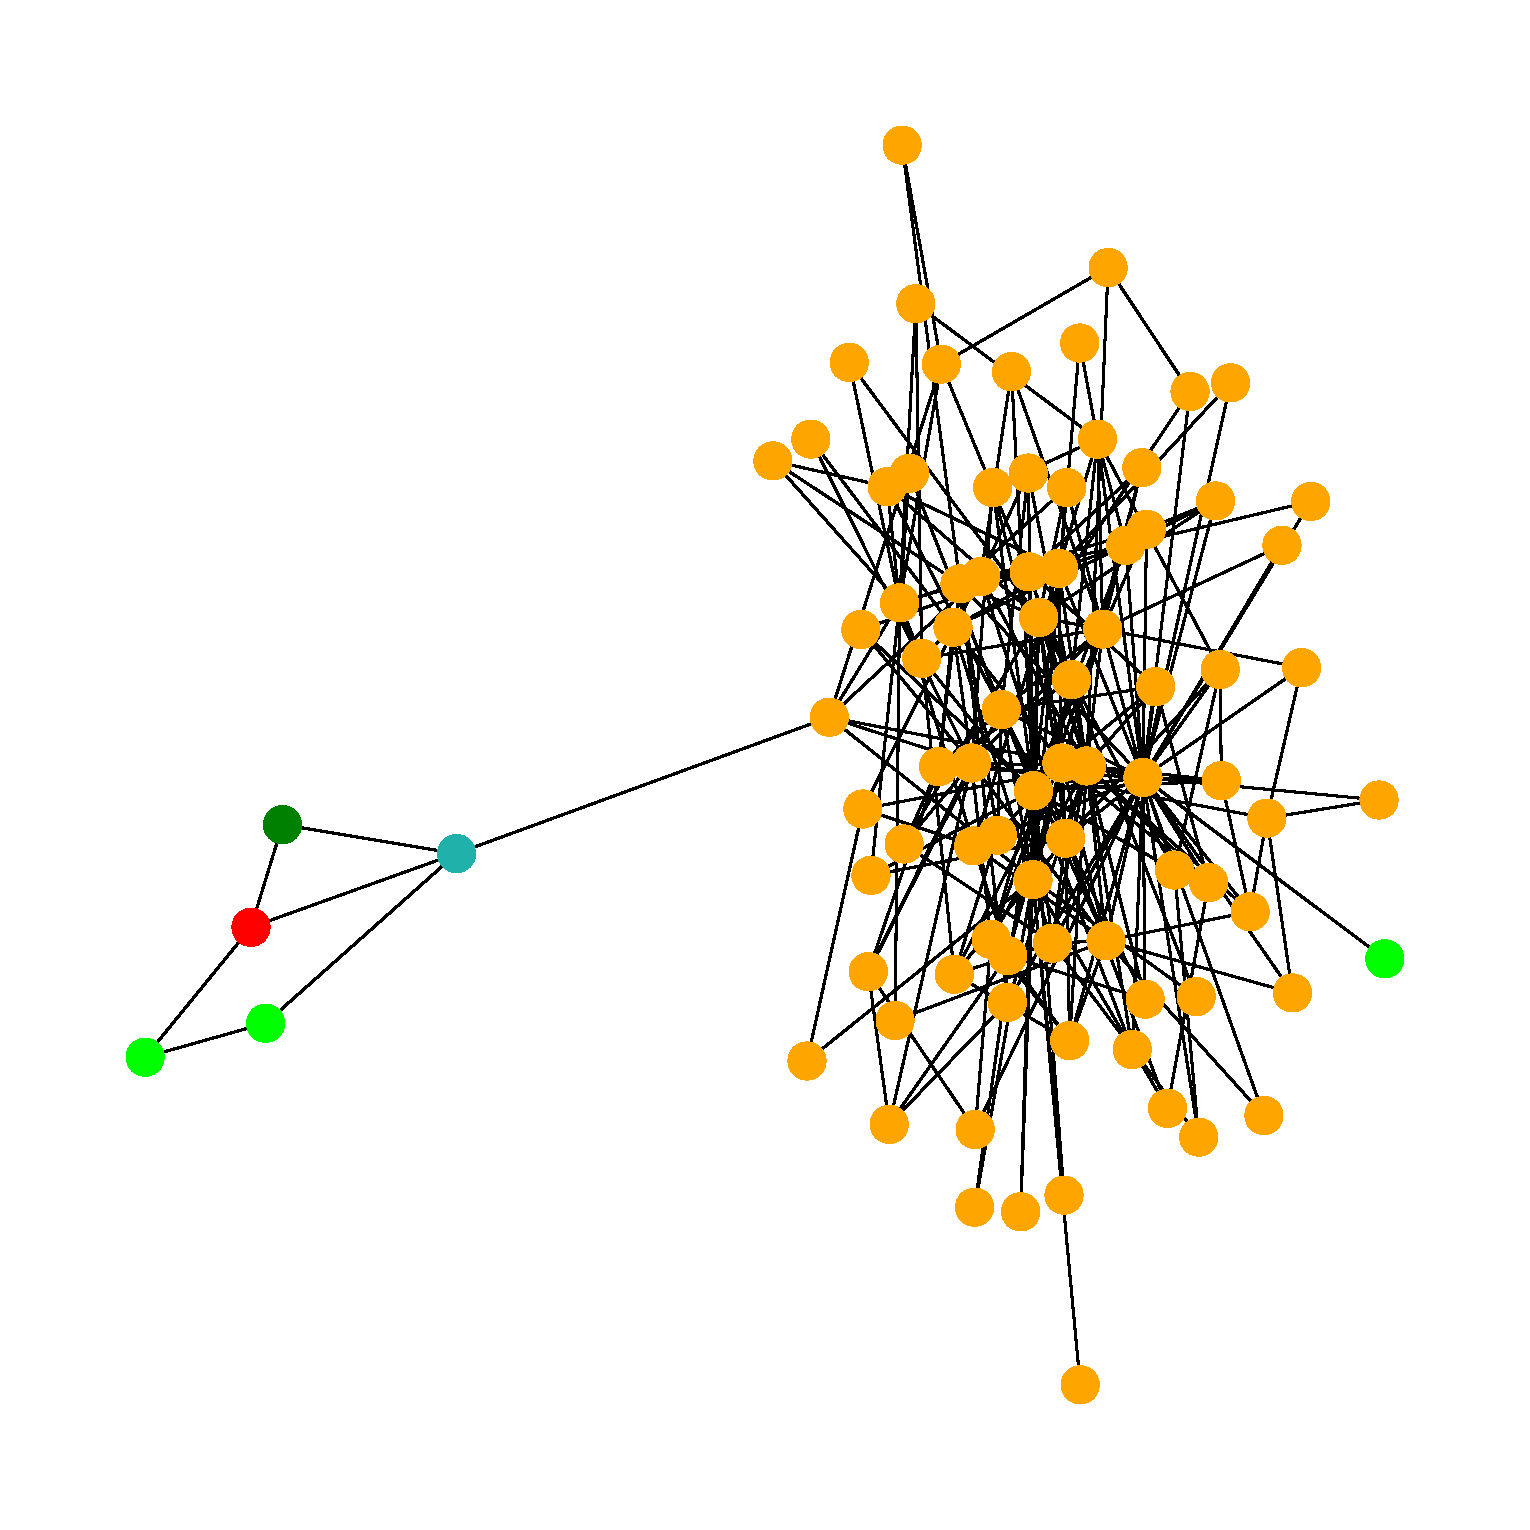
\includegraphics[width=\textwidth]{img/BA-Shapes-VIS-COMP-GRAPH.pdf}
        \caption{BA-Shapes}
    \end{subfigure}
    \hfill
    \begin{subfigure}[b]{0.4\textwidth}
        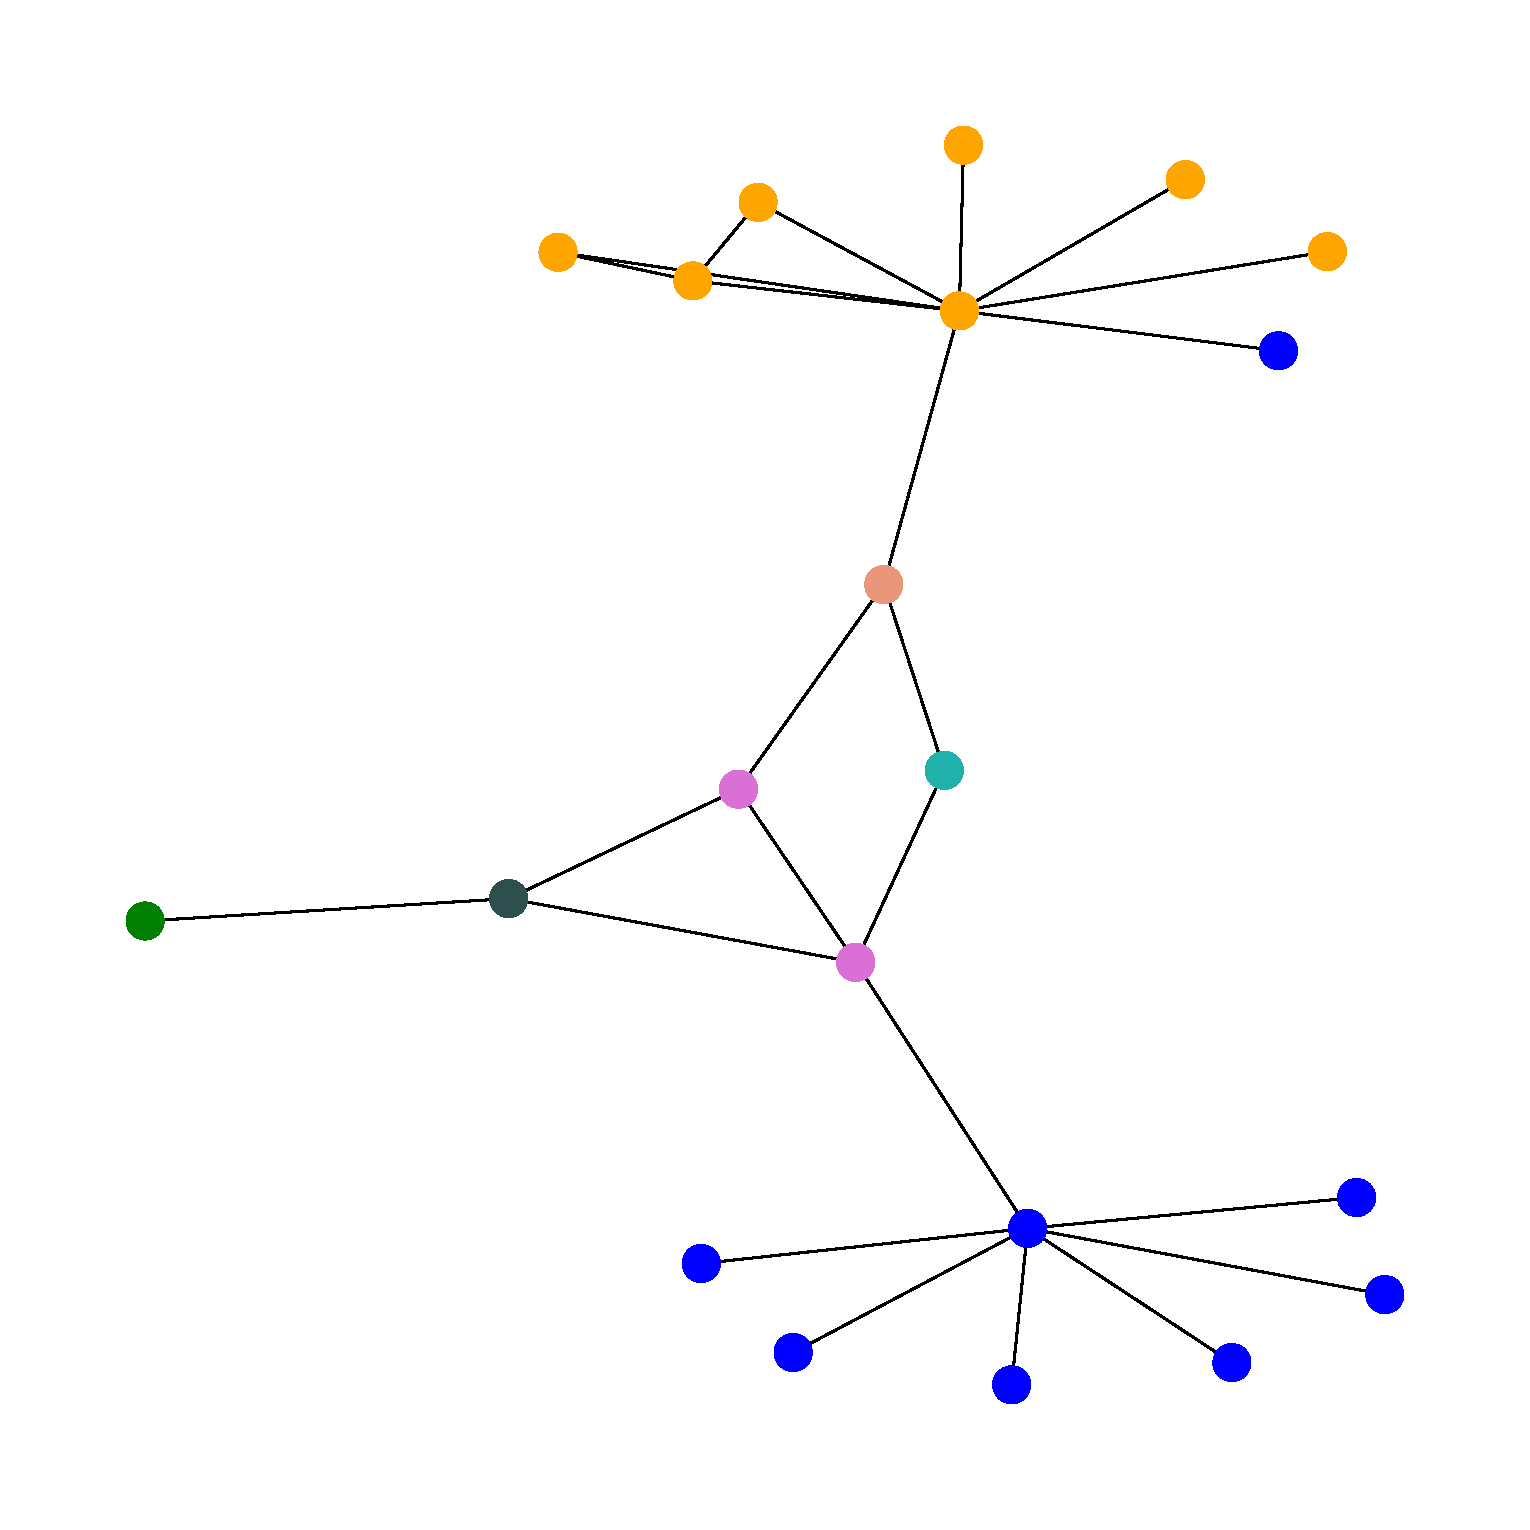
\includegraphics[width=\textwidth]{img/BA-Community-VIS-COMP-GRAPH.pdf}
        \caption{BA-Community}
    \end{subfigure}
    
    \vspace{0.5cm}
    
    \begin{subfigure}[b]{0.4\textwidth}
        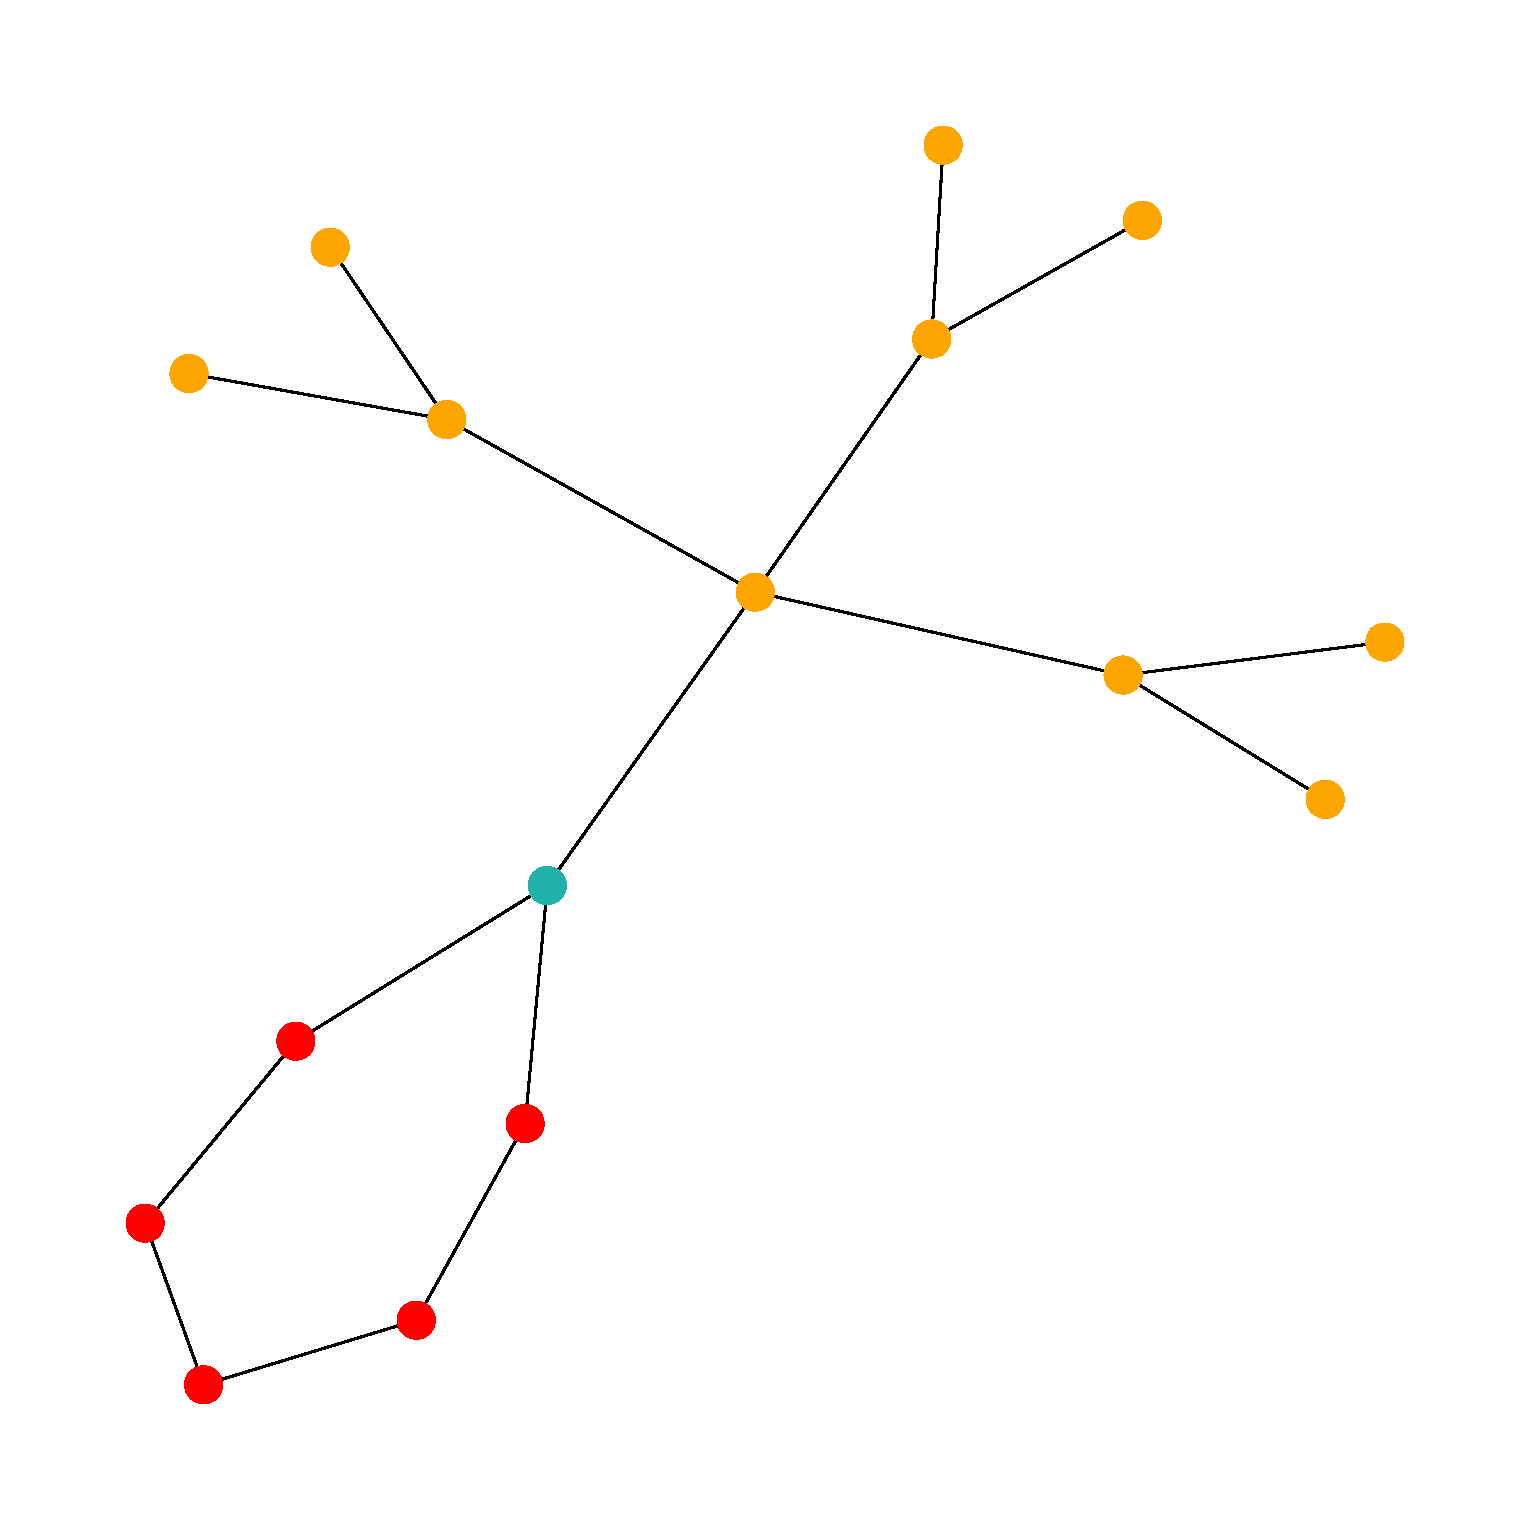
\includegraphics[width=\textwidth]{img/Tree-Cycles-VIS-COMP-GRAPH.pdf}
        \caption{Tree-Cycles}
    \end{subfigure}
    \hfill
    \begin{subfigure}[b]{0.4\textwidth}
        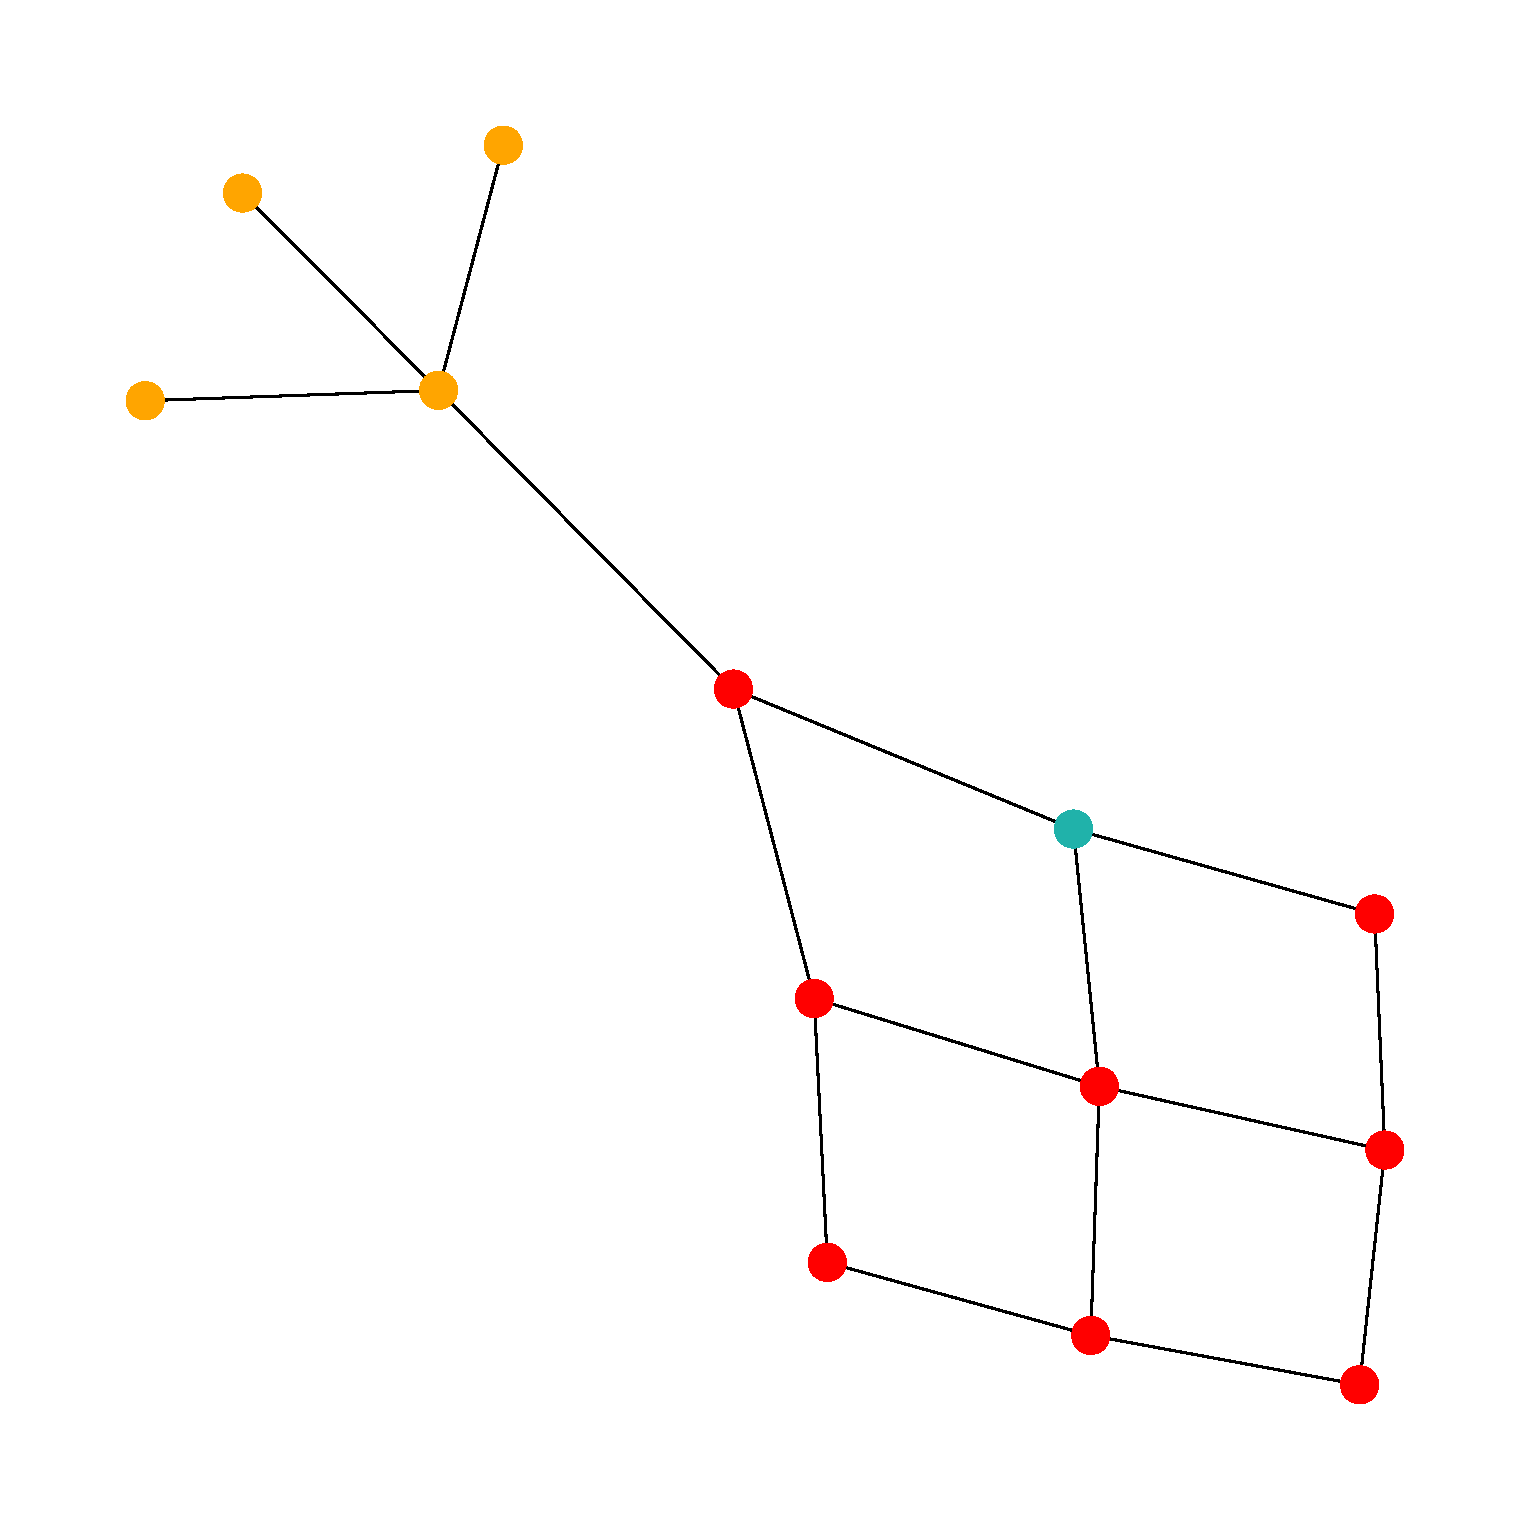
\includegraphics[width=\textwidth]{img/Tree-Grid-VIS-COMP-GRAPH.pdf}
        \caption{Tree-Grid}
    \end{subfigure}
    
    \vspace{0.5cm}
    
    \begin{subfigure}[b]{0.4\textwidth}
        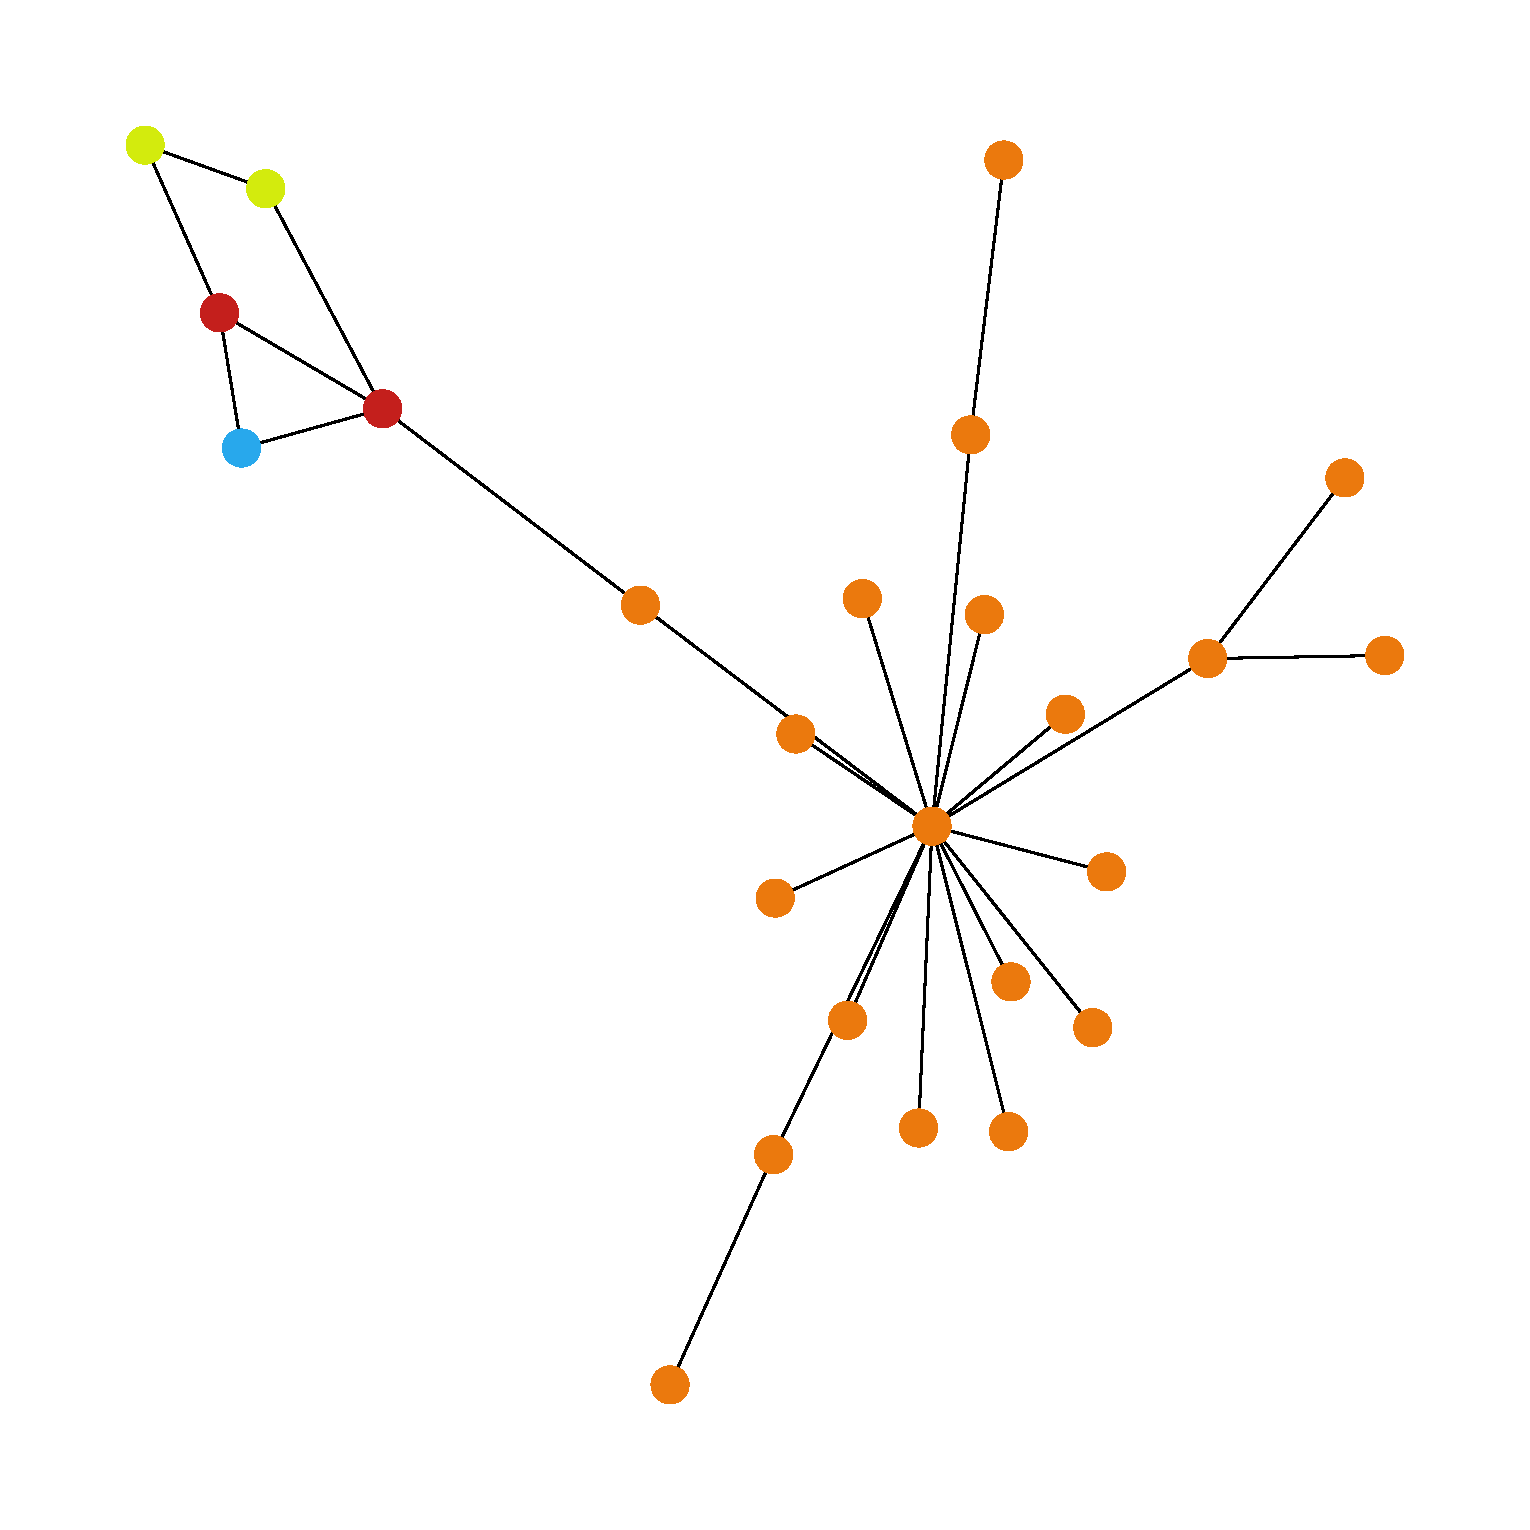
\includegraphics[width=\textwidth]{img/BA-2Motif-VIS-UNLABELED.pdf}
        \caption{BA-2Motif}
    \end{subfigure}
    \hfill
    \begin{subfigure}[b]{0.4\textwidth}
        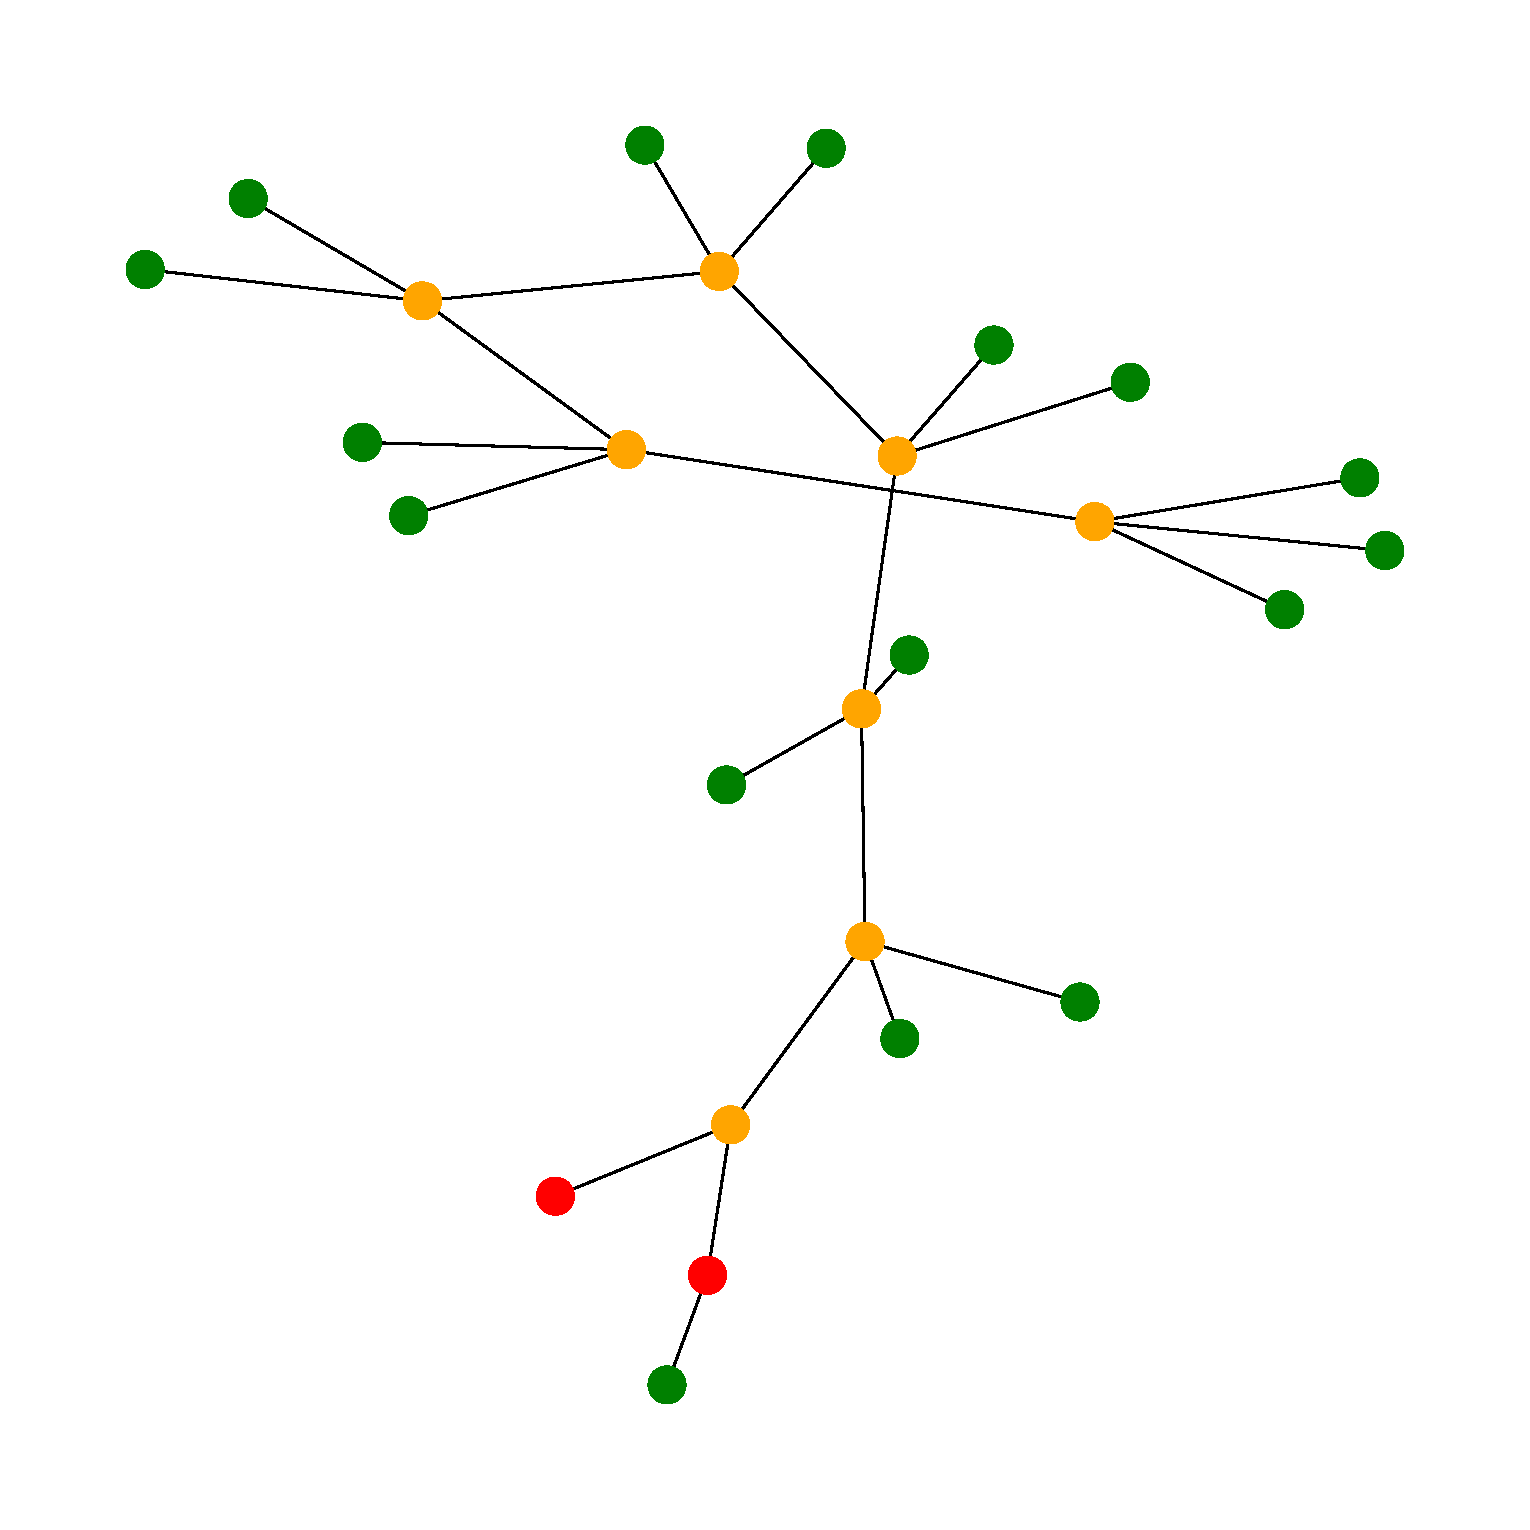
\includegraphics[width=\textwidth]{img/MUTAG-VIS-LARGE-UNLABELED.pdf}
        \caption{MUTAG}
    \end{subfigure}

    \caption[Visualization of original PGExplainer datasets]{Visualization of all six datasets. For node datasets the target node where the computational graph is computed from is colored in light blue.}
\end{figure}